%!TeX spellcheck = en-US
%!TEX root = CAN.tex
\documentclass[a4paper, 11pt]{article}

\usepackage{wrapfig}
\usepackage{graphicx}
\usepackage{graphics}
\usepackage{amsmath}
\usepackage{amsfonts}
\usepackage[T1]{fontenc}
\usepackage{amssymb}
\usepackage[font=footnotesize, singlelinecheck=false, labelfont=bf]{caption}
\usepackage{array}
\usepackage{multirow}
\usepackage{setspace}
\usepackage{hyperref}
\usepackage{verbatim}
\usepackage{epstopdf}
\usepackage{textcomp}
\usepackage{nicefrac}
\usepackage{xspace}
\usepackage{lineno}
\usepackage[footnotesize, bf, hang, raggedright]{subfigure}
\usepackage{charter}
\usepackage[expert]{mathdesign}
\usepackage[bottom]{footmisc}
\usepackage[english]{babel}
\usepackage{tikz}
\usepackage{multirow}
\usepackage{tabularx}
\usetikzlibrary{arrows}

\onehalfspacing
\usepackage[left=2.9cm,right=2.9cm,top=3cm,bottom=4.5cm]{geometry}

\newcommand{\subfigureautorefname}{\figurename}
\newcommand\geant{\textsc{Geant\,4}\xspace}
\newcommand\mokka{\textsc{Mokka}\xspace}
\newcommand\ddhep{\textsc{DD4hep}\xspace}

\usepackage{xcolor}
\usepackage[printwatermark]{xwatermark}
\newwatermark[allpages,color=gray!30,angle=45,scale=3,xpos=-10,ypos=0]{Draft}

\usepackage{titlesec}
\titleformat{\section}[hang]{
\usefont{T1}{qhv}{b}{n}\selectfont} % "qhv" - TeX Gyre Heros, "b" - bold
{}
{0em}
{\hspace{-0.4pt}\Large \thesection\hspace{0.6em}}

\usepackage[subfigure]{tocloft} % subfigure option only if using subfigure package
\renewcommand{\cfttoctitlefont} % ToC title
             {\usefont{T1}{qhv}{b}{n}\selectfont\huge}
\renewcommand{\cftsecfont} % section titles
             {\usefont{T1}{bch}{b}{n}\selectfont}
\renewcommand{\cftsubsecfont} % subsection titles
             {\usefont{T1}{bch}{m}{n}\selectfont}
\renewcommand{\cftsecpagefont} % section page numbers
             {\cftsecfont}
\renewcommand{\cftsubsecpagefont} % subsection page numbers
             {\cftsubsecfont}

\renewcommand{\arraystretch}{1.25}% Spread rows out...

\linenumbers
\setcounter{tocdepth}{2}


\begin{document}

%!TEX root = CAN.tex
\begin{titlepage}
\begin{flushright}
CALICE Analysis Note CAN-0XX\\
v1.0\\
\today\\
\end{flushright}

\begin{center}
\vspace*{\fill}
\begin{LARGE} \textbf{Timing Measurement in the CALICE Analog Hadronic Calorimeter engineering prototype} \end{LARGE} \\ [10ex]
\begin{Large} The CALICE Collaboration \footnote{Corresponding author: \\ Eldwan Brianne; eldwan.brianne@desy.de}\\ [10ex]
\end{Large}

\begin{large}
\textbf{Abstract} \\
\end{large}
\end{center}
This note presents the results obtained with the CALICE \emph{Analog Hadronic Calorimeter} engineering prototype at the SPS CERN testbeam campaign in 2015. The analysis presents the timing calibration and includes timing distributions for muon, electron and pion beams. The results are compared to several \geant version 10.1 physics lists.\\
\\

\textit{
This note contains preliminary CALICE results, and is for the use of members of the CALICE Collaboration and others to whom permission has been given.}

\end{titlepage}


%!TEX root = CAN.tex

\noindent\rule\textwidth{.1pt}
\tableofcontents
\noindent\rule\textwidth{.1pt}

\section{Introduction}

The International Large Detector (ILD) \cite{ILC_TDR} considers a highly granular hadronic calorimeter using iron absorbers to achieve a compact detector with the best jet energy resolution around 3-4\% at 250 GeV satisfying the space constrain imposed by the solenoid magnet. Timing measurements in a calorimeter can be used to reject out of time pile-up events. In addition, the high level of $\gamma\gamma \rightarrow$ hadrons background could be rejected by using timing information of the calorimeter in order to limit the impact of background events on physics measurements. Finally, time information could be used to improve the energy reconstruction \cite{IEEE_timing}.

A hadronic shower possesses several timing components related to different processes happening in the shower. A fast component related to instantaneous highly energetic deposits from high-energy hadrons and electromagnetic sub-showers. A slow component due to neutron scattering, nuclear-recoil and photons from nuclear processes, this component can last up to several milliseconds. Apart from physics processes, the measured hit time is influenced by the active medium used as well as the front-end electronics. Time constants in the active medium such as the scintillation decay time can affect the time measurement.

The performance of the ILD relies on simulation studies based on \geant. It is important to study how well the simulation performs to reproduce the time structure of hadronic showers observed in data. The CALICE Analog Hadronic Calorimeter (AHCAL) technological prototype has been installed in the SPS CERN facilities in July 2015 in order to provide measurements using plastic scintillators. The goal of this study is to improve our knowledge about hadronic showers especially about its time evolution and time correlations of layers within the calorimeter. This note presents the time calibration procedure of the AHCAL and the results obtained in muon, electron and pion beams in an energy range from 10 GeV to 90 GeV, as indicated in table \ref{table:dataruns}.

\section{Testbeam Setup}

The testbeam setup at CERN in July 2015, at the SPS beamline H1, is shown in figure \ref{fig:TestbeamScketch}. The AHCAL is composed of 48 iron absorber plates in which 14 active layers are installed. The AHCAL detector is placed on a movable stage in order to be able to move the detector position relative to the beam for muon calibration runs.

\begin{figure}[htbp!]
	\centering
	\includegraphics[width=0.7\linewidth]{fig/TestbeamSetup.pdf}
	\caption{Sketch view of the beamline setup at the CERN SPS H1 beamline in July 2015.} \label{fig:TestbeamScketch}
\end{figure}

The beam instrumentation consists of two $10\times10$ cm$^2$ scintillator plates in front of the calorimeter, and two $50\times50$ cm$^2$ scintillator plates, one placed in front of the calorimeter and one placed at the back of the calorimeter. They are read-out by photomultiplier tubes. The coincidence of the $50\times50$ cm$^2$ scintillator plates is used for the muon runs and the coincidence of the $10\times10$ cm$^2$ scintillator plates is used for the electron and pion runs as a trigger signal. Additionally, the coincidence signal from the scintillator is provided directly to several channels of the AHCAL in order to provide a reference time information of the trigger as shown in table \ref{table:trigger_ref}. A Cherenkov detector, at around 100 m upstream, was available to tag incoming particles.

\begin{table}[htb!]
	\centering
	\caption{List of runs taken at SPS in July 2015.}
	\label{table:dataruns}
	\begin{tabular}{@{}lp{2cm}p{7.5cm}p{2cm}@{}}
		\toprule
		\multicolumn{1}{l}{\textbf{Particle}} & \textbf{Energy} & \textbf{Runs} & \textbf{\# Events}\\
		\midrule
		\multirow{2}{*}{$\mu^-$}& 50 GeV & 24016-24204 & 120,887,651\\& 150 GeV & 24623-24662 & 15,534,328\\
		\midrule
		\multirow{2}{*}{e$^-$}& 10 GeV & 24531-24576 & 38,028,438\\& 15 GeV & 24507-24527 & 7,701,325\\& 20 GeV & 24479-24504 & 10,498,554\\& 30 GeV & 24454-24475 & 3,382,943\\& 40 GeV & 24420-24448 & 2,665,843\\& 50 GeV & 24404-24419 & 5,933,995\\
		\midrule
		\multirow{2}{*}{$\pi^-$}& 10 GeV & 24266-24272, 24300-24317, 24381-24397 & 24,311,420\\& 20 GeV & 24398-24400 & N/A\\& 30 GeV & 24259-24299, 24319-24380 & 10,120,753\\& 50 GeV & 24212-24254, 24325-24357, 24580-24612 & 10,704,661\\& 70 GeV & 24219-24242, 24365-24374 & 8,885,407\\& 90 GeV & 24233-24287, 24331-24364 & 7,955,604\\
		\bottomrule
	\end{tabular}
\end{table}

\begin{table}[htb!]
	\centering
	\caption{List of AHCAL channels used as time reference for this analysis. In this analysis, the time reference signals T$_{12}$, T$_{13}$ and T$_{14}$ are used.}
	\label{table:trigger_ref}
	\begin{tabular}{@{} ccccc @{}}
		\toprule
		Layer \# & Chip Number & Channel & Comments & Name \\
		\midrule
		11 & 169 & 29 & noisy & T$_{11}$ \\
		11 & 177 & 23 & broken & - \\
		12 & 185 & 29 & - & T$_{12}$ \\
		13 & 201 & 29 & -  & T$_{13}$ \\
		13 & 211 & 6 & broken & - \\
		14 & 217 & 23 & - & T$_{14}$ \\
		\bottomrule
	\end{tabular}
\end{table}

\section{Simulation}

\subsection{Geometry implementation}

The simulation of the testbeam prototype is based on the \mokka \cite{MoradeFreitas:2002kj} framework v08-05-01 and the new \ddhep \cite{Frank:2014zya} framework v00-16, which both provide a full \geant v10.1 based simulation of the detector with detailed geometry and material descriptions. A right-handed coordinate system is used such that the Z-axis points in the beam direction and that the Y-axis is directed upwards. No beamline instrumentation is simulated except scintillator triggers in front of and behind the detector. An additional layer of 5.6 mm of lead (corresponds to 1 $X_0$) is added in front of the calorimeter in order to account for missing upstream material. This additional material was determined using the electron data and matching the simulation with the center of gravity distribution in the z-direction.

This analysis uses the sub-detector \mokka models \textit{TBecal4d} for the ScECAL (Scintillator strips with EBUs) and \textit{TBhcal4d} for the AHCAL. The distance between the sub-detectors is set to 0 mm. The absorber structure is square-shaped in simulation, on contrary wedge-shape in reality, but it is not expected to have any influence. The placement of the active layers are the following: 2 single EBU boards, 8 single HBU boards and 4 $2\times2$ HBU boards (in slots 11, 13, 21, 31 of the absorber structure).

The simulation includes also saturation effects in the scintillator known as the Birk's Law. The saturation appears a high ionization densities due to shielding effects of the scintillator material. The implementation of the Birk's Law in \geant is used. A check was performed with \mokka and \ddhep models with muons and electrons to ensure that the material description in both models is better than 20\%.

The beam gun is placed 1 m in front of the calorimeter face for the simulations in this analysis. It is configured to generate single beam particles with a 2\% momentum spread, according to the beamline, and the beam profile for electrons and pions is extracted from data and applied to simulation. For muon runs, a flat beam covering the full AHCAL is simulated as this is not expected to have an influence on the MIP and time response of the detector. All electron simulations are simulated with \geant v10.1 using the QGSP\_BERT\_HP physics list.

Pion showers are simulated using QGSP\_BERT, QGSP\_BERT\_HP and QBBC physics lists. The package \textit{high precision} (\_HP) is used in order to understand the differences induced in timing with a precise treatment of the neutrons.

\subsection{Digitization}

The digitization of simulated hits is very similar to the one used in the ScECAL and AHCAL physics prototypes \cite{2011_JINST_6_P04003}. First, the energy deposited in a cell is converted in MIP. This is done in order to have the simulation on the same energy scale as the testbeam data once converted. The conversion unit named \textit{MIPtoGeV} is extracted from simulation by projecting 8 GeV muons onto the AHCAL detector and fitting the resulting spectrum of the deposited energy. Motivated by physics, ideally for a thin active material, the energy deposited follows a Landau distribution. The most probable value (MPV) of this distribution is used as the \textit{MIPtoGeV} factor. For this thesis, a value of 470 keV is used for the AHCAL and 309 keV for the ScECAL.

If available, individual calibration factors obtained from data are used to extract the light yield which is needed to model the statistical fluctuations of photons hitting a SiPM \cite{Hartbrich:2016bbz}. Saturation effects are also included using the number of pixels available on each SiPM type. Most of the tiles used are wrapped with a reflective foil such that crosstalk effects between channels can be neglected. For layers with no wrapping, a default value of 15\% cross-talk is applied.

Additionally, noise needs to be taken into account for the engineering AHCAL prototype. It is important to note that noise is much lower than in the physics prototype but it is important to be taken into account for this thesis as timing is very sensitive to low statistics late tails. Noise is added using muon runs by removing found tracks and keeping remaining hits.

The timing is modeled in the same way as in the SPIROC, the energy from sub-hits in a cell is integrated over a sliding time window of 15 ns, if the energy sum passes the threshold, the time of the simulated sub-hit is used as the time of the hit. In order to simulate detector resolution effects, the time of a hit is smeared with a double Gaussian function with slightly different means and sigmas convoluted with a Gaussian of fixed mean and variable sigma.

After digitization, simulated hits have the same format as raw data hits and are then reconstructed using the same software chain as is used for data. To suppress noise, only hits above 0.5 MIP are considered in this analysis in both simulation and data.

\subsection{Model Validation}

\section{Event Selection}

\subsection{Muon selection}

To select muons, an event pre-selection and a track finder \cite{} selection is performed. A cut on the number of hits in the AHCAL is done at 20 as the number of hits should be around 1 per layer for a MIP-like particle plus the number of noise hits expected in the detector. The track finder algorithm selects AHCAL towers of hits in the same $x:y$ position and it rejects AHCAL towers that contains less than a certain number of hits. In order to select muons or punch-through pions, a straight track of at least 7 hits is required in the whole AHCAL. This assumes that the calorimeter was perfectly perpendicular to the beam, therefore any tilted tracks would be missed. In addition, to reject late pion showers, no more than 2 hits are allowed per layer to account for some flexibility with noise hits.

\subsection{Electron selection}

Electron events are needed to validate the timing behavior in simulation as well as the detector simulation model. It is important to have a clean sample of electrons to cross-check the timing calibration. An electron selection is done using the beam instrumentation and layer information. Events with a Cherenkov tag are used. The energy deposit in the first three AHCAL layers ($E_3+E_4+E_5$) must be over 10 MIPs. A box cut on the number of hits and the center of gravity in the z direction is done. As the number of hits in a electron shower is proportional to the shower energy, this cut is energy dependent. The energy deposited in the last two layers relative to the energy deposited in the calorimeter ($(E_{13}+E_{14})/\Sigma E$) is required to be under 1\% to reject pion showers and to contain the electron shower.

\subsection{Pion selection}

The goal of the pion selection is to reject punch-through pions, muons and possible electron contamination as these events would be instantaneous. The events without a Cherenkov tag are selected. The number of hits required per event needs to be over 20 to reject most muons or punch-through pions without cutting on the center of gravity in z in order not to bias the start of the pion shower. The energy fraction deposited in the two last AHCAL layers must be over 1\% in order to ensure that pion showered and reject possible electron showers. The number of hits in the two first AHCAL layers $N_3+N_4$ must be under 5 to mitigate possible particle contamination from electrons.

\section{Timing calibration of the AHCAL}

In a first time, the muon data is used to determine the parameters for the timing calibration. Muons are used because the process they induce is instantaneous. In a second step, the calibration is cross-checked using the electron data as also EM showers are instantaneous. This enables a verification of the time calibration procedure and may reveal effects that are not present in the muon data.

\subsection{Time recording in the SPIROC2b}

The time information provided by the SPIROC2b \cite{} in the data is in TDC units. Similar to the ADC scale, it would be difficult to compare directly channels using the TDC unit. The TDC information needs to be interpreted into a common unit of time, the nanosecond. The TDC information of each channel can be converted into nanoseconds following the simple schematic shown in figure \ref{fig:ConvertTime}.

\begin{figure}[htbp!]
  \centering
  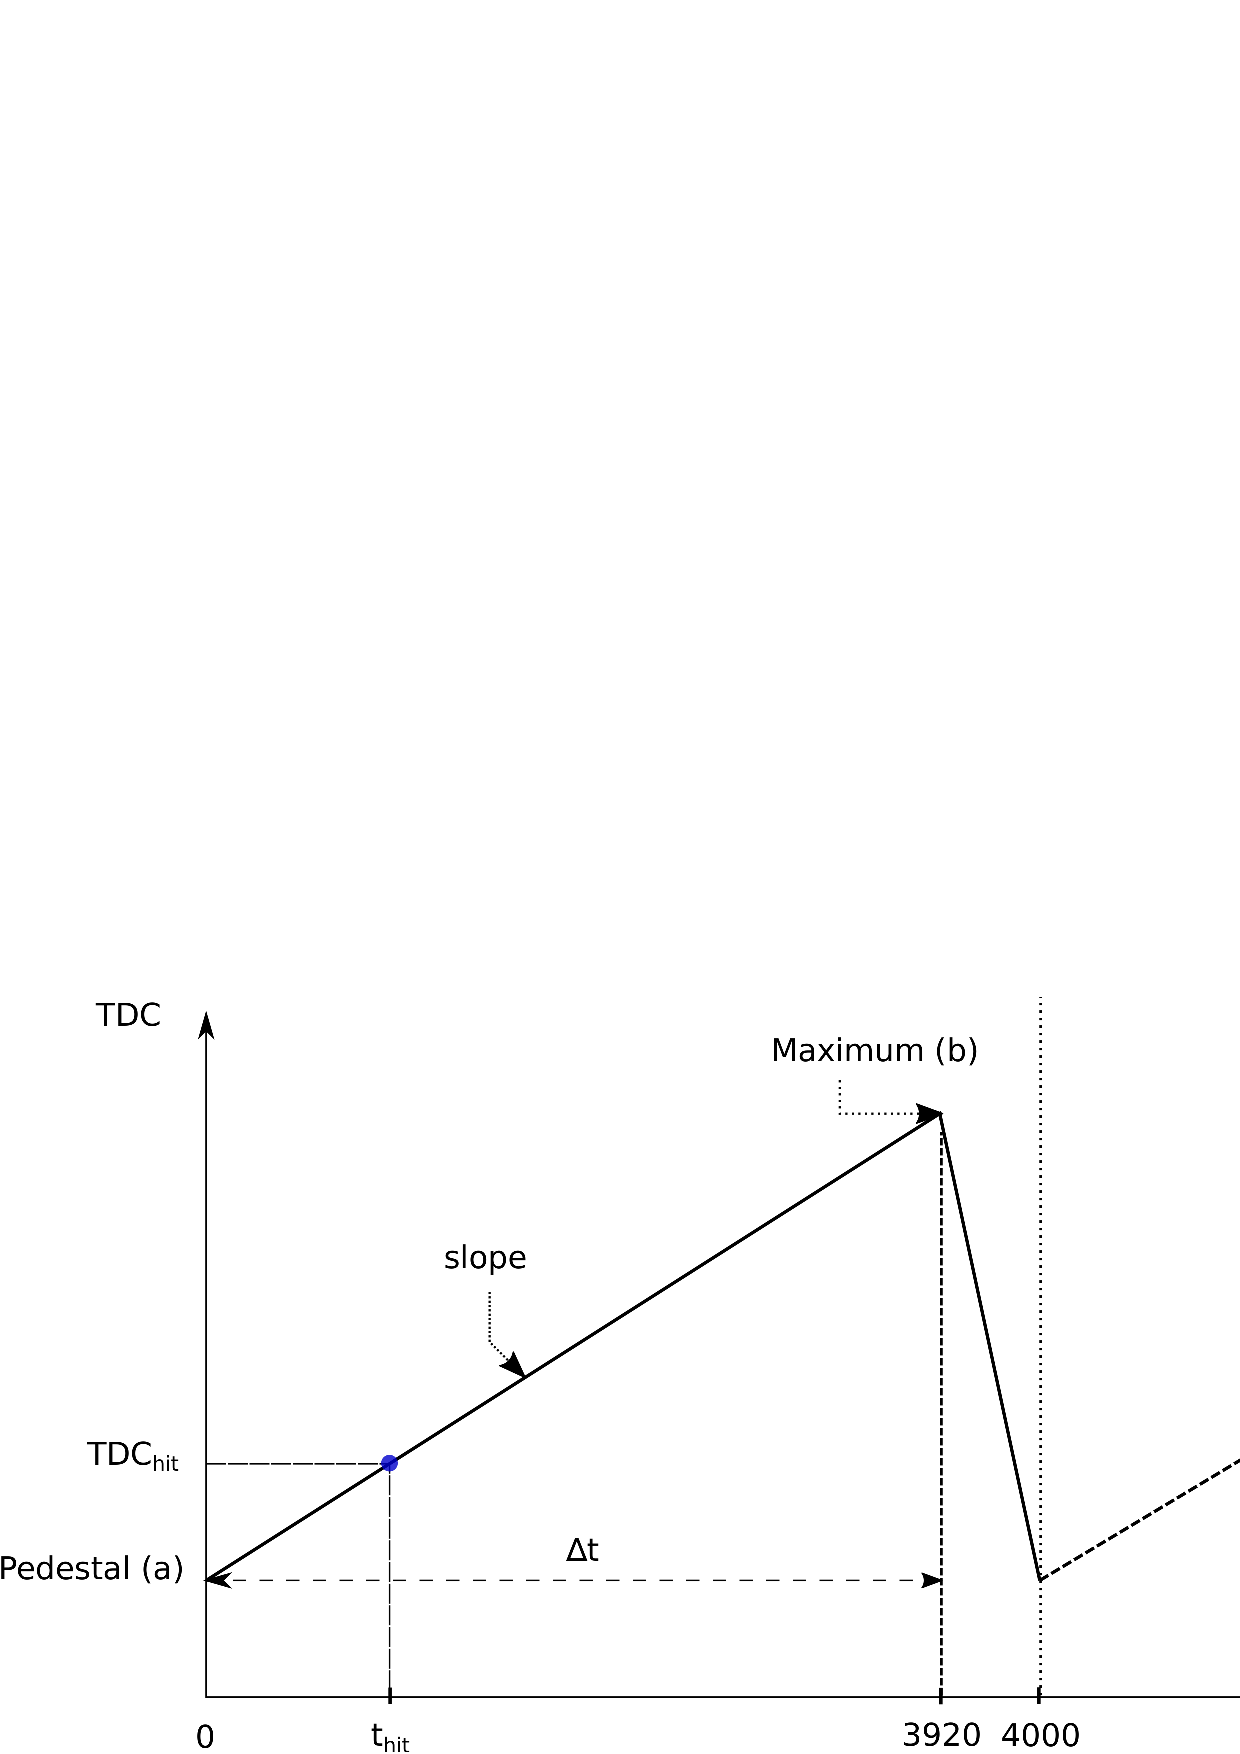
\includegraphics[width=0.9\linewidth]{fig/TDCRamp.pdf}
  \caption{Schematic of the TDC ramp in the SPIROC2b used in testbeam with a slow clock of 250 kHz. The slope of the ramp is $\Delta_t$/(Max-Ped). The time of the hit is then calculated as the following: t$_{Hit}$ = slope $\times$ (TDC$_{Hit}$ - Ped).} \label{fig:ConvertTime}
\end{figure}

In order to determine the ramp slope, the starting point or pedestal of the ramp and the endpoint of the ramp are measured. Since the SPIROC2b has two TDC ramps, each defined by a BXID parity (even or odd), two slopes need to be extracted per chip. In addition, each channel can store up to 16 events called memory-cell. Each memory-cell is different thus 16 calibration values or pedestal are needed per channel. The extraction of the slope and the determination of the pedestal is described in the following sections.

\subsection{Timing calibration procedure}

The timing calibration procedure of the AHCAL is quite tedious and requires a lot of steps. An overview of the steps performed for the time calibration of each individual AHCAL channels is shown in figure \ref{fig:CalibOverview}.

\begin{figure}[htbp!]
  \centering
  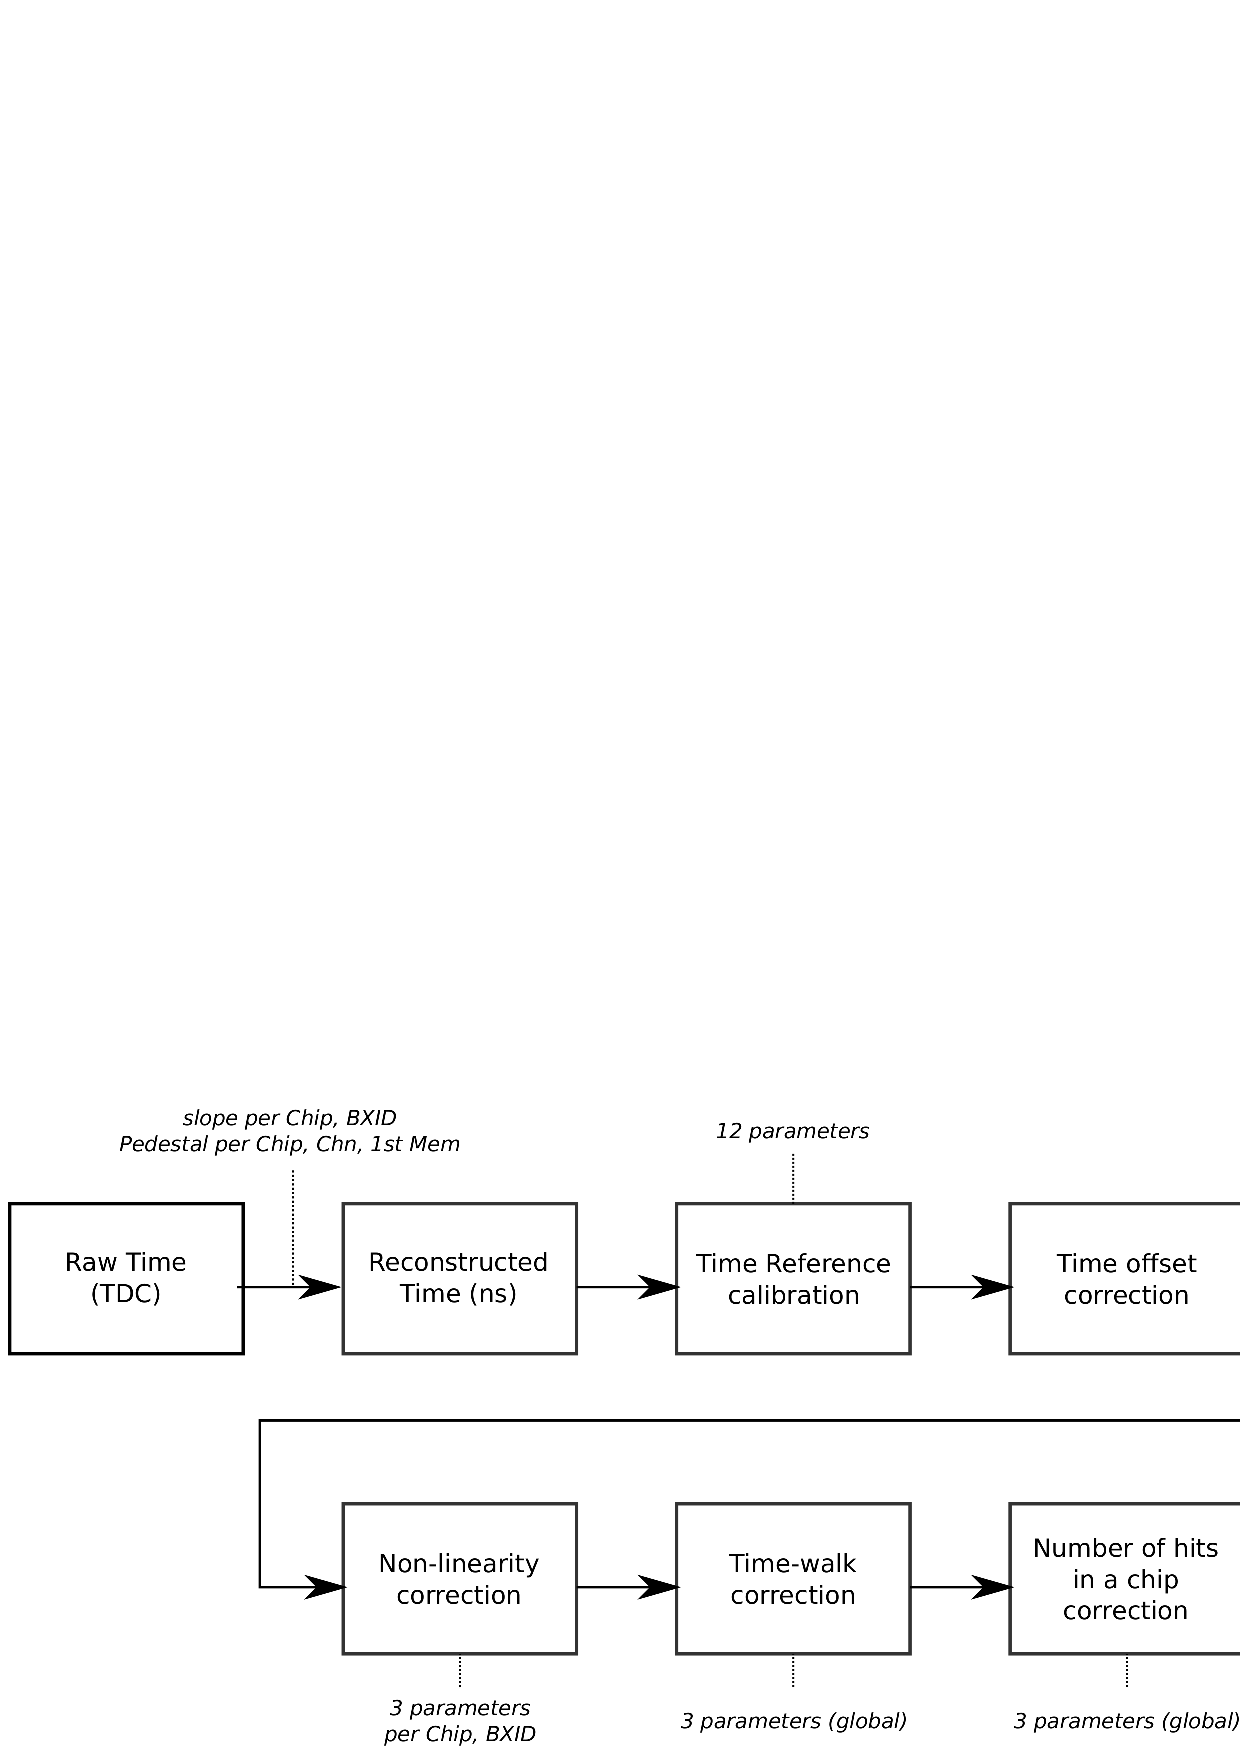
\includegraphics[width=1\linewidth]{fig/TimeCalibOverview.pdf}
  \caption{Overall view of the different steps performed for the AHCAL timing calibration. In total, more than 20000 constants are needed.} \label{fig:CalibOverview}
\end{figure}

\subsection{Slope and Pedestal extraction}

To reconstruct the time in a channel, the TDC value measured needs to be converted into nanoseconds. The slope is calculated as
\begin{equation} \label{eq:slope}
	s \: \text{[ns/TDC]} = \frac{3920}{a - b}
\end{equation}
where $s$ is the TDC ramp slope, $a$ is the endpoint of the TDC ramp and $b$ is the start point of the TDC ramp that is referred in the following as the pedestal. The total length of the ramp is 3920 ns instead of the expected value of 4000 ns due to a deadtime of around 2\% \cite{Brianne2012} induced by the multiplexer that switches between the two ramps.

\begin{figure}[htbp!]
	\begin{subfigure}[t]{0.49\textwidth}
		\centering
		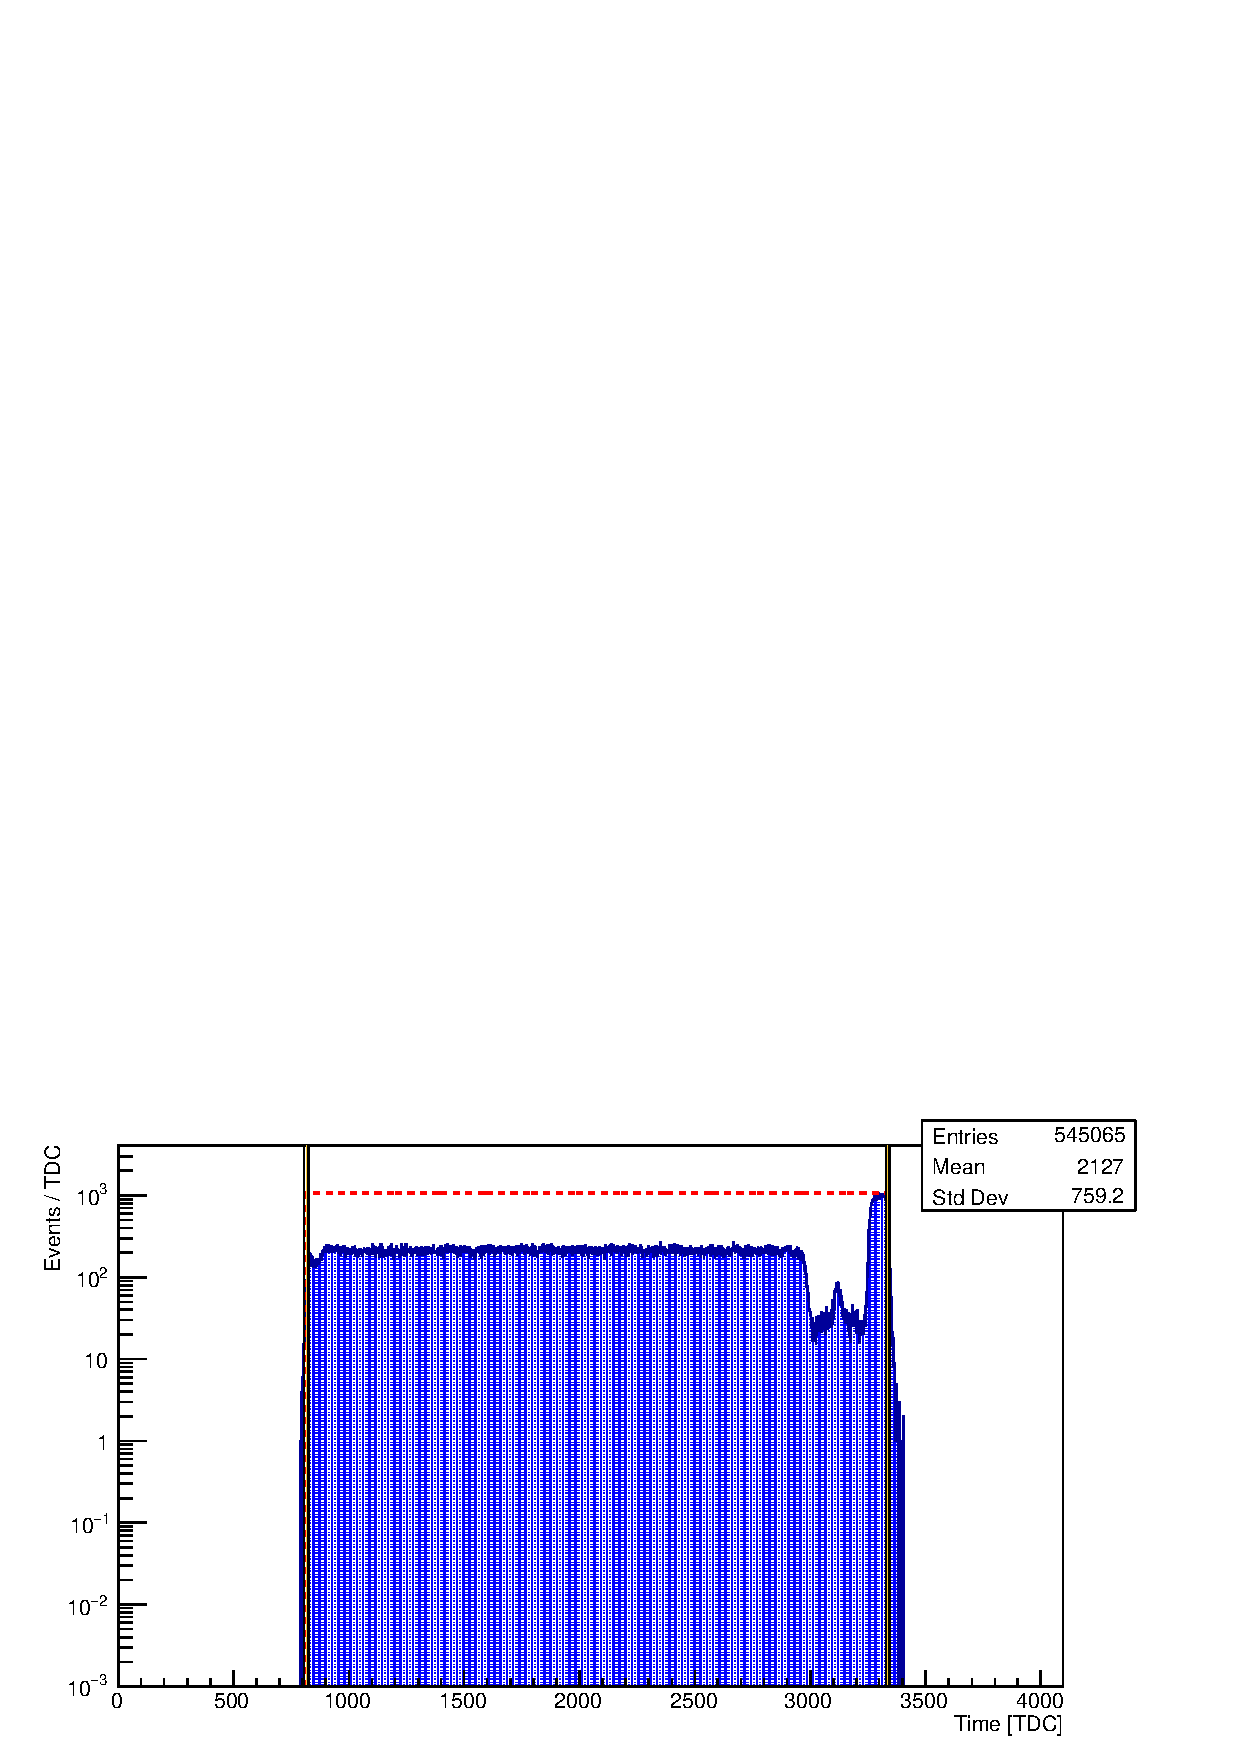
\includegraphics[width=1\linewidth]{fig/ExampleTDCSpectra.pdf}
		\caption{} \label{fig:TDC_Spectrum}
	\end{subfigure}
	\hfill
	\begin{subfigure}[t]{0.49\textwidth}
		\centering
		\includegraphics[width=1\linewidth]{fig/SlopesTDC.pdf}
		\caption{} \label{fig:slopes}
	\end{subfigure}
	\caption{\subref{fig:TDC_Spectrum}) TDC spectrum of a typical chip. The black lines indicate the fitted Max and Pedestal parameters for this chip. The yellow bands represent the uncertainty on the extraction of the parameter $a$ and $b$. The extracted parameters are $s$ = 1.47 $\pm$ 0.01 ns/TDC, $b$ = 888 $\pm$ 5 TDC and $a$ = 3613 $\pm$ 8 TDC. \subref{fig:slopes}) Distribution of the fitted slopes for even and odd bunch-crossing IDs. $\mu_{odd}$ = 1.564 ns/TDC, RMS$_{odd}$ = 0.121, $\mu_{even}$ = 1.556 ns/TDC, RMS$_{even}$ = 0.113. In total, 208 TDC slopes were extracted.}
\end{figure}

At a first order, the slope of the TDC ramp is assumed to be linear. The parameters $a$ and $b$ are extracted from the TDC spectrum of a channel per chip and BXID parity using only the first memory-cell as shown in figure \ref{fig:TDC_Spectrum}. The TDC ramp slope does not depend on the memory-cell as the memory-cell only introduce an offset on the parameters $a$ and $b$. A total of 208 slopes have to be extracted for the testbeam setup.

The extracted values for the slopes are shown in figure \ref{fig:slopes}. They are in the expected range of 1.6 ns per TDC bin due to the limited dynamic range provided by the chip, around 2500 TDC bins for 4 $\mu$s.

\subsection{Time delay correction}

The time reference of the trigger is delayed compared to the muon passing through the detector because the length of cables and the trigger electronics logic. Therefore, the time offset of the time reference is determined from data. Muons are instantaneous particles thus the time of the first hit distribution for each channel, memory cell and BXID should peak at 0 ns.

\begin{figure}[htbp!]
	\centering
	\includegraphics[width=0.6\textwidth]{fig/Timing_Chip236_Chn21_Mem01_BXID1_withOffset.pdf}
	\caption{Time of first hit distribution for a single channel (Chip 236, Chn 21, Mem 01, BXID 1). An offset of -165.2 ns is determined for this channel.}\label{fig:TimeChnwithOffset}
\end{figure}

A shifting procedure of the time of the hit relative to the time reference for each channel, memory-cell and BXID parity is performed. This is done to take into account the delay time of the trigger due to cabling and the trigger electronics as well as possible differences in channel pedestals. Only memory-cells containing more than 100 events are considered. The histogram range of the time of the hit relative to the time reference is reduced iteratively until the RMS of the distribution is under 10 ns. This value was chosen because it corresponds to more than 3 sigma of the time reference uncertainty. The mean of the histogram is then used as the time offset value. An example of a single channel is shown in figure \ref{fig:TimeChnwithOffset}.

In total, 21040 individual offsets are extracted from data. The mean value of the time offset is around -150 ns which is around the expected value considering the cabling length and the trigger logic delay.

\subsection{Non-linearity correction}

The time calibration relies on the linearity of the TDC voltage ramp in the \textit{SPIROC2B}. This assumption is not entirely reliable as described in \cite{Hartbrich2011, Brianne2012}. The voltage slope shows a slight kink around the middle thus leading to a non-linear ramp. For this, a correction of the non-linearity is applied. Since the time reference is determined from a non-linear TDC ramp and it can't be corrected due to the lack of external time reference, the position of $T_{hit}$ - $T_{ref}$ on the ramp is corrected. The non-linearity correction results in an improvement in the timing resolution (RMS) of the AHCAL by about 5.1\%.

\subsection{Time-walk correction}

The time-walk effect is due to the presence of an energy threshold that induces a time shift between a small amplitude signal and a high amplitude signal. Small amplitude signals will systematically trigger at a later time than high amplitude signals for a shaper that makes the signals peak at the same time. A time correction is determined by looking at the time of the first hit as a function of the amplitude of the hit. This may be particularly relevant for late energy depositions in hadron showers that comes generally from neutrons depositing little energy in the calorimeter. An improvement of around 3\% is achieved on the time resolution of the AHCAL.

\begin{figure}[htbp!]
	\centering
	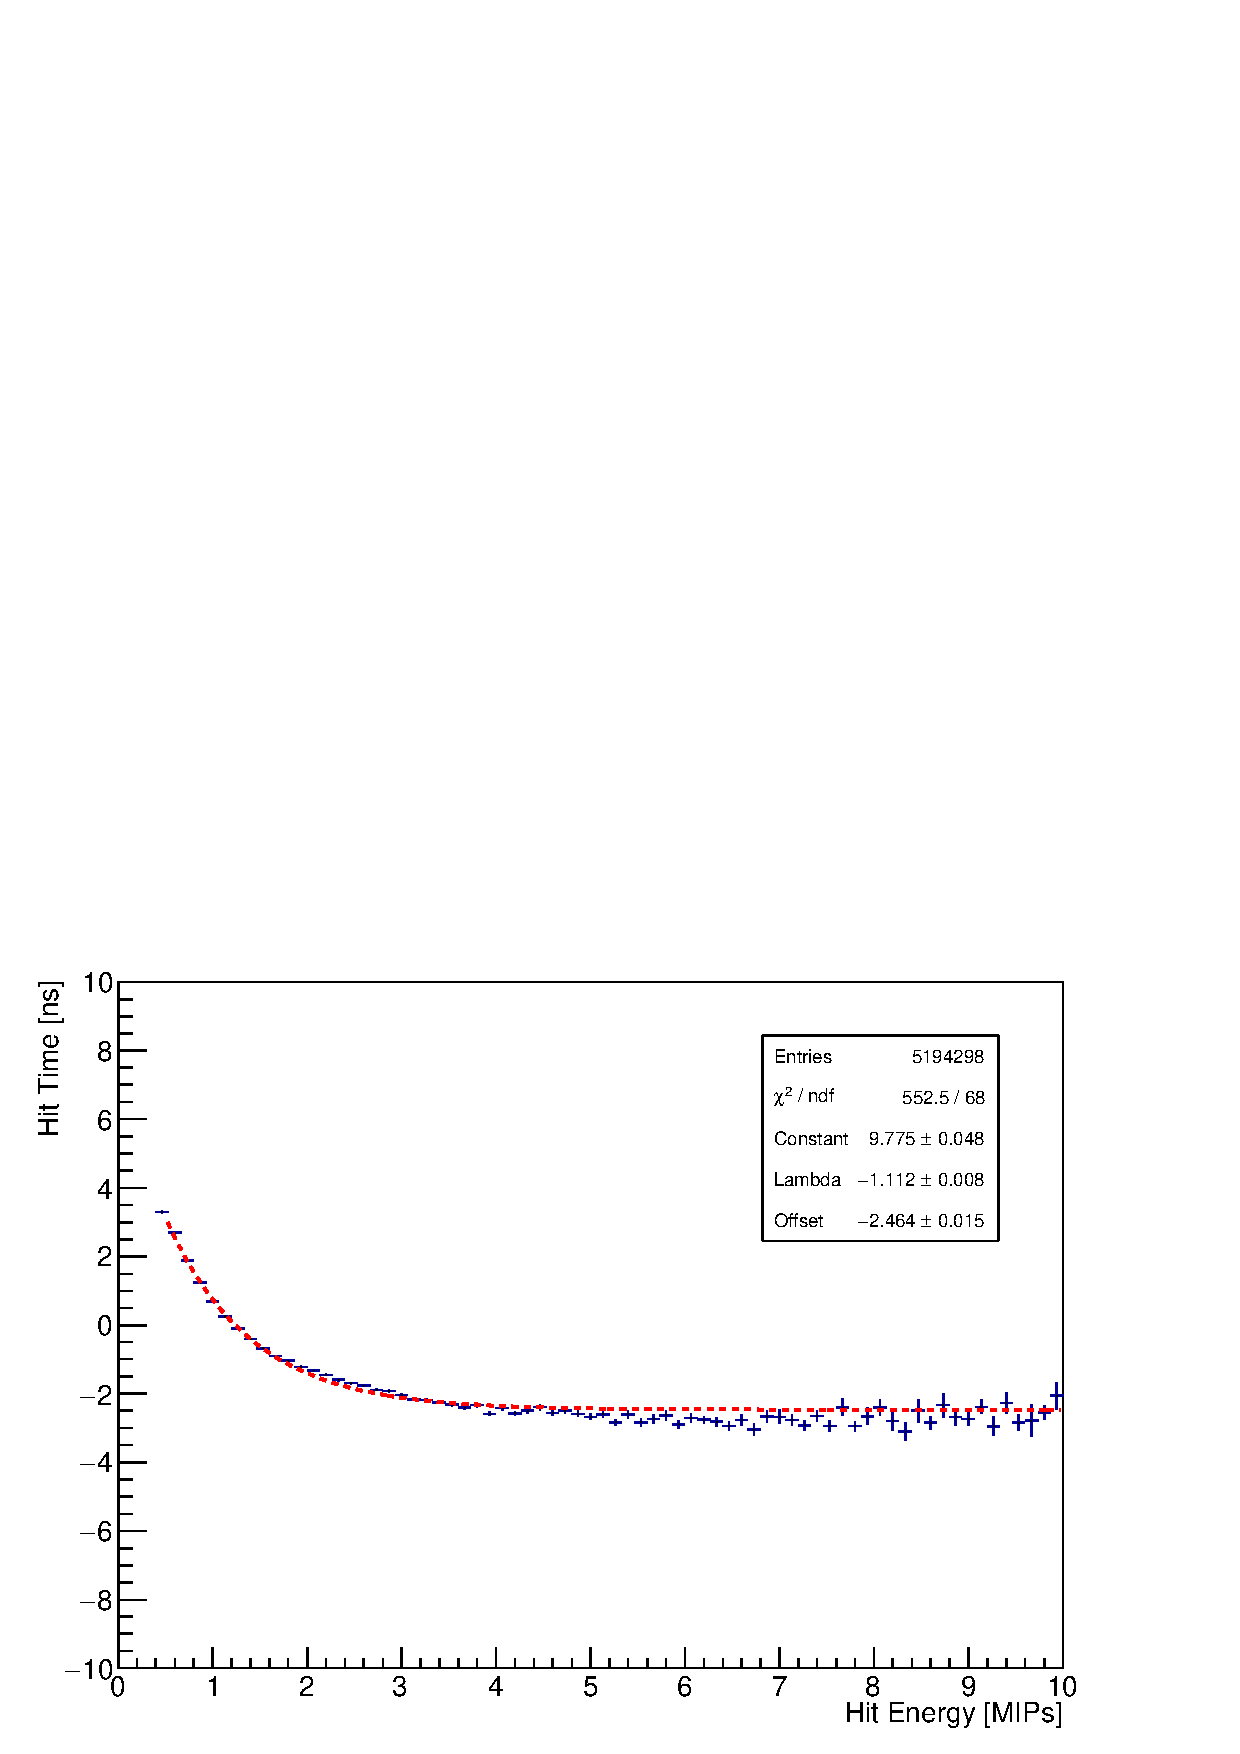
\includegraphics[width=0.6\textwidth]{fig/TimeWalkProfile.pdf}
	\caption{Time of first hit as a function of the hit energy. A difference up to 6 ns is seen between small and large amplitudes. Time-walk correction extracted from data. The fit function is of the form $\text{A} \times e^{-\lambda{}x} + \text{B}$.}\label{fig:time_walk}
\end{figure}

\subsection{Number of triggered channel in a chip correction}

The mean time of first hit as a function of the number of triggered channels over 0.5 MIP in a chip is shown in figure \ref{fig:nhits_profile}. A time shift up to 20-40 ns can be seen depending on the number of triggered channels in a chip. The cause of the observed effect is most likely due to an element in the chip called a \textit{delay box} that gets unstable with a high charge going through the chip. This chip element is responsible for the hold signal of the TDC ramp in the chip. The hold signal is delayed, and thus a higher TDC ramp value than the one expected is sampled.

\begin{figure}[htbp!]
	\centering
	\includegraphics[width=0.6\textwidth]{fig/NumberHits_Dependance_AllEnergies.pdf}
	\caption{Mean time of the first hit as a function of the number of triggered channels above 0.5 MIP in a chip. The mean time shift upwards with the increase of triggers leading to large tails in the time distribution. A second order polynomial fit is done for the time correction shown by the red dashed line.}\label{fig:nhits_profile}
\end{figure}

In order to determine a reliable time correction, the time correction parameters are determined combining all the electron data. This effect may be chip-dependent and the parameters for the correction may differ from chip to chip. However, the limited amount of data does not allow to determine a correction function for each chip. Therefore, a global function is used to correct the time in the data.

\section{Results}

\subsection{Systematic uncertainties}

\subsection{Timing of muon and electron beams}

\subsection{Timing of pion showers}

\section{Conclusion}

%!TEX root = CAN.tex
\addcontentsline{toc}{section}{Bibliography}
\begin{thebibliography}{10}
\bibitem{ILC_TDR}
T.Behnke and al., \textit{The International Linear Collider Technical Design Report - Volume 4: Detectors}, \\
arXiv:1306.6329v1
\bibitem{IEEE_timing}
	A. Benaglia and al., \textit{Space-Time Development of Electromagnetic and Hadronic Showers and Perspectives for Novel Calorimetric Techniques}, \\
	IEEE TNS Vol.63-2, doi:10.1109/TNS.2016.2527758
\bibitem{SPSBeamLine}
	CERN, \textit{Secondary Beam \& Areas}, \\
	\href{http://sba.web.cern.ch/sba/BeamsAndAreas/h2/H2manual.html}{http://sba.web.cern.ch/sba/BeamsAndAreas/h2/H2manual.html}
\bibitem{CAN-038}
	The CALICE Collaboration, \textit{The Time Structure of Hadronic Showers in Tungsten and Steel with T3B}, \\
	CALICE Analysis Note CAN-038
\bibitem{AHCAL_Physics}
	The CALICE Collaboration, \textit{Validation of GEANT4 Monte Carlo models with a highly granular scintillator-steel hadron calorimeter}, \\
	2013 JINST 8 P07005, doi:10.1088/1748-0221/8/07/P07005
\bibitem{SPIROCManual}
	Omega Group, \textit{SPIROC Manuel}, \\
	\href{http://omega.in2p3.fr/index.php/download-center/doc_view/165-spiroc2-datasheet.raw?tmpl=component}{http://omega.in2p3.fr/index.php/download-center/doc\_view/165-spiroc2-datasheet.raw?tmpl=component}
\bibitem{OskarSSP}
	 O. Hartbrich, \textit{Investigation of the time measurement capabilities of the SPIROC2b ASIC}, \\
	 DESY summer student report, 2011.
\bibitem{EldwanSSP}
	 E. Brianne, \textit{Studies of the front-end electronics of the Analog HCAL}, \\
	 DESY summer student report, 2012.
\bibitem{OskarMaster}
	 O. Hartbrich, \textit{Commissioning and LED System Tests of the Engineering Prototype of the Analog Hadronic Calorimeter of the CALICE Collaboration}, \\
	 DESY-thesis-2012-040, ISSN 1435-8085.
\bibitem{CAN-002}
	 The CALICE Collaboration, \textit{First results from electron data with the CALICE tile HCAL prototype at the CERN test-beam}, \\
	 CALICE Analysis Note CAN-002
\bibitem{CAN-010}
	 The CALICE Collaboration, \textit{Electron data with the CALICE tile AHCAL prototype at the CERN test-beam - Update}, \\
	 CALICE Analysis Note CAN-010
\bibitem{JINST-6}
	 The CALICE Collaboration, C. Adloff et al., \textit{Electromagnetic response of a highly granular hadronic calorimeter}, \\
	 2011 JINST 6 P04003, doi:10.1088/1748-0221/6/04/P04003
\bibitem{DAQ}
	 T. Suehara and al., \textit{AIDA-CALICE DAQ interface} \\
	 AIDA 2020 Scientific/Technical Note, AIDA-2020-NOTE-2016-006
\end{thebibliography}


\section{Additional figures}


\bibliography{biblio}
\clearpage

\begin{appendix}

	\section*{Appendix}
  \addcontentsline{toc}{section}{Appendix}

	\begin{table}[htb!]
		\centering
		\caption{List of runs taken at SPS in July 2015.}
		\label{table:dataruns}
		\begin{tabular}{@{}lp{2cm}p{7.5cm}p{2cm}@{}}
			\toprule
			\multicolumn{1}{l}{\textbf{Particle}} & \textbf{Energy} & \textbf{Runs} & \textbf{\# Events}\\
			\midrule
			\multirow{2}{*}{$\mu^-$}& 50 GeV & 24016-24204 & 120,887,651\\& 150 GeV & 24623-24662 & 15,534,328\\
			\midrule
			\multirow{2}{*}{e$^-$}& 10 GeV & 24531-24576 & 38,028,438\\& 15 GeV & 24507-24527 & 7,701,325\\& 20 GeV & 24479-24504 & 10,498,554\\& 30 GeV & 24454-24475 & 3,382,943\\& 40 GeV & 24420-24448 & 2,665,843\\& 50 GeV & 24404-24419 & 5,933,995\\
			\midrule
			\multirow{2}{*}{$\pi^-$}& 10 GeV & 24266-24272, 24300-24317, 24381-24397 & 24,311,420\\& 20 GeV & 24398-24400 & N/A\\& 30 GeV & 24259-24299, 24319-24380 & 10,120,753\\& 50 GeV & 24212-24254, 24325-24357, 24580-24612 & 10,704,661\\& 70 GeV & 24219-24242, 24365-24374 & 8,885,407\\& 90 GeV & 24233-24287, 24331-24364 & 7,955,604\\
			\bottomrule
		\end{tabular}
	\end{table}

	\begin{table}[htb!]
		\centering
		\caption{List of AHCAL channels used as time reference for this analysis. In this analysis, the time reference signals T$_{12}$, T$_{13}$ and T$_{14}$ are used.}
		\label{table:trigger_ref}
		\begin{tabular}{@{} ccccc @{}}
			\toprule
			Layer \# & Chip Number & Channel & Comments & Name \\
			\midrule
			11 & 169 & 29 & noisy & T$_{11}$ \\
			11 & 177 & 23 & broken & - \\
			12 & 185 & 29 & - & T$_{12}$ \\
			13 & 201 & 29 & -  & T$_{13}$ \\
			13 & 211 & 6 & broken & - \\
			14 & 217 & 23 & - & T$_{14}$ \\
			\bottomrule
		\end{tabular}
	\end{table}

	\begin{table}[htb!]
		\centering
		\caption{Selection cuts for the muon runs.}
		\label{table:muon_sel}
		\begin{tabular}{@{}lll@{}}
			\toprule
			\multicolumn{1}{l}{\textbf{Name}} & \textbf{Beam Energy} & \textbf{Cut}\\
			\midrule
			\multirow{2}{*}{Preselection}& All & 0 mm < $cog_{z}$ < 800 mm\\& All & 0 < $n_{hits}$ < 20 \\
			\multirow{2}{*}{Track Selection SSF}& All & $n_{hits}$ in tower > 7 \\& All & $n_{hits}$ in layer < 3 \\
			\multirow{2}{*}{Track Selection BL}& All & $n_{hits}$ in tower > 2 \\& All & $n_{hits}$ in layer < 3 \\
			\bottomrule
		\end{tabular}
	\end{table}

	\begin{table}[htb!]
		\centering
		\caption{Selection cuts for each electron runs.}
		\label{table:electron_sel}
		\begin{tabular}{@{}lll@{}}
			\toprule
			\multicolumn{1}{l}{\textbf{Name}} & \textbf{Beam Energy} & \textbf{Cut}\\
			\midrule
			\multirow{2}{*}{Event Quality}& All & Cherenkov ON\\& All & Energy in the first 3 layers of AHCAL > 10 MIP \\
			\multirow{9}{*}{Electron Selection}& 10 GeV & 25 < $n_{hits}$ < 75 \\& 15 GeV & 30 < $n_{hits}$ < 90 \\& 20 GeV & 40 < $n_{hits}$ < 100 \\& 30 GeV & 50 < $n_{hits}$ < 110 \\& 40 GeV & 60 < $n_{hits}$ < 120 \\& 50 GeV & 70 < $n_{hits}$ < 140 \\& All & $cog_{z}$ < 250 mm\\& All & -90 mm < $cog_{x, y}$ < 90 mm \\& All & Energy in last two layers < 1\% $E_{sum}$ \\
			\bottomrule
		\end{tabular}
	\end{table}

	\begin{table}[htb!]
		\centering
		\caption{Selection cuts for the pions runs.}
		\label{table:pion_sel}
		\begin{tabular}{@{}lll@{}}
			\toprule
			\multicolumn{1}{l}{\textbf{Name}} & \textbf{Beam Energy} & \textbf{Cut}\\
			\midrule
			\multirow{1}{*}{Event Quality}& All & Cherenkov OFF\\
			\multirow{3}{*}{Pion Selection}& All & $n_{hits}$ > 20 \\& All & $n_{hits}$ in the first 2 AHCAL layers < 5 \\& All & Energy in last two layers > 1\% $E_{sum}$ \\
			\multirow{2}{*}{Multi Particle Rejection}& All & $n_{hits}$ in time window > 5 \\& All & $n_{Cluster}$ > 0 \\
			\bottomrule
		\end{tabular}
	\end{table}

\end{appendix}

\end{document}
